% Writeup for MDS
% David Lawrence Miller
% d.l.miller@bath.ac.uk
  
\documentclass[a4paper,10pt]{article}
\setlength{\textheight}{22.5cm}
\setlength{\textwidth}{6.47in}
\setlength{\oddsidemargin}{-1mm}
\setlength{\topmargin}{0.1cm}
\setlength{\evensidemargin}{-5mm} 
 
% Load some packages
\usepackage{times, amsmath, amssymb, amsfonts, url, natbib, bm, rotating}
 
\usepackage{multirow}
\usepackage{graphicx}
\usepackage{rotating}

% top matter
\title{Multidimensional scaling as a tool for smoothing over complex regions}
\author{David Lawrence Miller\\Mathematical Sciences\\University of Bath\\\texttt{d.l.miller@bath.ac.uk}}
 
% Shortcuts
% Probability
\newcommand{\prob}[1]{\mathbb{P}\left[ #1 \right]}
% Schwarz-Christoffel
\newcommand{\sch}{Schwarz-Christoffel }
% fprime
\newcommand{\fprime}{f^\prime(z)}
% figure reference command
\newcommand{\fig}[1]{\emph{fig.} \ref{#1}}
% Figure reference command
\newcommand{\Fig}[1]{\emph{Fig.} \ref{#1}}
% equation reference command
\newcommand{\eqn}[1]{\emph{eqn.} (\ref{#1})}
% phi inverse
\newcommand{\phiinv}{\phi^{-1}}
% use other phi
\renewcommand{\phi}{\varphi}
%transpose
\newcommand{\tr}[1]{#1^{\text{T}}}
% diagonal
\newcommand{\diag}{\text{diag}}
% call \times \cross
\newcommand{\cross}{\times}


\begin{document}
 
% The abstract
%\begin{abstract}
%Here.
%\end{abstract}
 
 
% New theorem for theorems
\newtheorem{thm}{Theorem}[section]
 
%New theorem for definitions
\newtheorem{defn}{Definition}[section]
 
\maketitle

%\markright{TECH. DETAILS OF SCHWARZ-CHRISTOFFEL MAPPING}

\section{Introduction}

\subsection{Motivation}

Generalized additive models (GAMs) are a popular way of performing spatial smoothing. In this context, they are used to fit smooth functions of location over a geographical region. A typical application of this is in ecological modeling; particularly when the population density of a species is sought. In this case the locations of observations of animals are recorded and fed into the model which can then be used to perform inference on the population, whether that be an abundance estimate, density map or a more sophisticated inferential goal.

When the geographical region has a complex boundary then features from one part of the domain can unduely influence other parts. This phenomenon is known as leakage. A typical example of this can be seen in \fig{leakage}. Leakage is problematic since it causes incorrect estimates of the density surface. This can then lead to incorrect abundance estimates, which is clearly not desirable.

The cause of leakage can be thought of in two ways: that the smooth does not respect the boundary conditions of the domain, or the smooth not taking into account the geometry of the domain; in particular with regard to the distance between points in the domain. Previous work in this area has been to combat leakage along these two lines. Work of \cite{ramsay} and \cite{soap} try to use boundary conditions to prevent leakage, where as \cite{wangranalli} attempt to approximate the within-area distances.

% leakage example 
\begin{figure}
\centering
% trim order l b r t
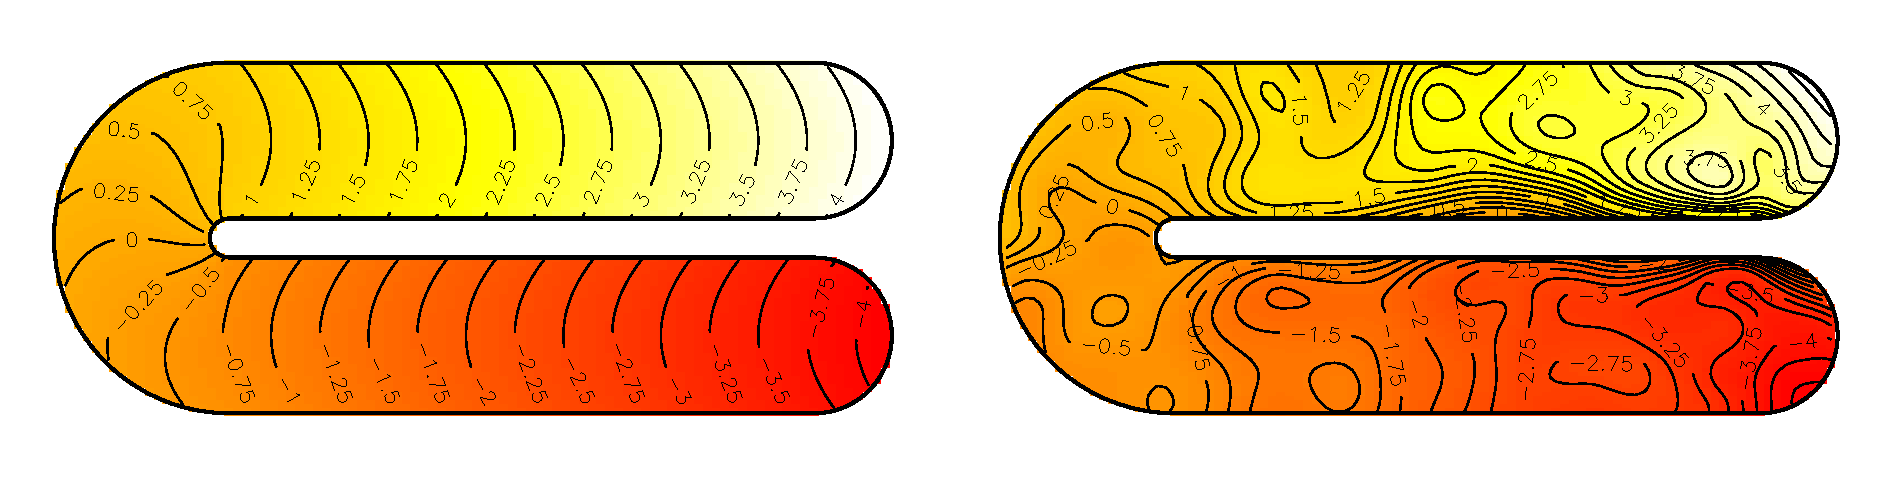
\includegraphics[width=4in]{figs/ramsay-leak.pdf}\\
\caption{An example of leakage. A thin plate spline basis was fit to the function on the left, here the model smooths accross the gap in the middle of the domain (right.)}
\label{leakage}
\end{figure}


\subsection{Proposition}

Multidimensional scaling (MDS) or, as it is often referred to, principle coordinates (PCO) is a method commonly used in multivariate analysis. MDS relocates the points such that although their coordinates have changed the distances between points are preserved (\cite{chatfieldcollins}, p. 187.) In this new configuration, the Euclidean inter-point distances are approximately the same as their distances in the original data. Most often, MDS is used as a dimension reduction technique, finding a projection of data into lower dimensional space, while still retaining information about the distances between the points. It is closely related to techniques such as PCA (\cite{chatfieldcollins}, p. 200) and canonical correspondence analysis (\cite{terbraak}.)

Multidimensional scaling offers an obvious framework for the problem of smoothing over a region with a complex boundary. We can use the within-area distances to configure the points such that the distances between the points are (approximately) preserved.

The modelling strategy is take the observations and the boundary of the domain, find the pairwise within-area distances for the observations and then perform MDS on the inter-observation distances, thus obtaining a new configuration of the data. Using this new configuration of the data, we fit the GAM. Inference can then be performed using this model. Should predictions be required then the those points at which predictions are needed should be inserted into the MDS configuration.

The rest of this report is structured as follows: in section 2 an overview of MDS is given, along with technical details of how the MDS configuration is calculated; section 3 focuses on how the within-area distances are found; section 4 shows some examples of this method on simulated data. I conclude with a proposed course of action to improve the method.

\section{Multidimensional Scaling}

The basic concept behind MDS is to take the data, calculate their inter-point distances and then find a new coordinate system based on those inter-point distances. We do this by simply performing an eigen-decomposition on the matrix of distances between points.

\subsection{Finding the new point configuration}

We first define $d_{ij}$ as the distance between the points $i$ and $j$. These form a (symmetric) matrix, $D$, with $ij^{\text{th}}$ element $d^2_{ij}$. In our case, we would like $d_{ij}$ to be the shortest distance between the points, given the path between the points remains within the domain. Finding $d_{ij}$ is discussed in the next section, for the moment let us assume that $D$ is known and gives the shortest within-domain distance between points.

\cite{diaconis08} gives a clear definition of the algorithm (due to \cite{schoenberg35}) for finding the new locations of points given we know the $d_{ij}$s which is outlined below.

First, suppose that the $n$ the unknown locations (in $n$ dimensions) in our new configuration are entries in an $n \times n$ matrix, $\tilde{X}$. Let $S=\tilde{X}\tr{\tilde{X}}$. Then performing an eigen-decomposition such that $S=U\Lambda\tr{U}$, where $U$ is the $n \cross n$ matrix of eigenvectors and $\Lambda$ is the $n \cross n$ diagonal matrix of eigenvalues.

Then, since $S$ is symmetric, we are interested in:
\begin{equation}
\tilde{X}=U\Lambda^{\frac{1}{2}}.
\end{equation}
We can relate $D$ to $S$ by first defining:
\begin{equation}
H = I-\frac{1}{n}\mathbf{1}\tr{\mathbf{1}}.
\end{equation}
By pre- and post-multiplying any matrix by $H$ we double centre it (such that row and column means are 0.) We then obtain:
\begin{equation}
S = -\frac{1}{2}HDH.
\end{equation}
See \cite{diaconis08} for a simple proof of this.

Following these steps $\tilde{X}$ is an $n \cross n$ matrix. The aim here is two smooth in two dimensions, so, the directions with the two largest eigenvalues are chosen to represent the space. This gives the two dimensional representation of the data, taking into account the within-area distance. From here on $\tilde{X}$ refers to the $n \cross 2$ dimensional matrix obtained from truncating the full new coordinate set to the first two columns (in eigenvalue order.)

So, in order to obtain a the new configuration of points using MDS (given that we have some set of inter-point distances) we merely need to double centre the matrix of distances and perform an eigen-decomposition on the resulting matrix, $S$. 

Note that an additive constant can be computed and added to the non-diagonal entries of $D$ to ensure that the eigenvalues of $S$ are non-negative.

Multidimensional scaling may be performed in \textsf{R} using the \texttt{cmdscale} function. 

\subsection{Gower's interpolation} 

It is likely that we may be in a position where the coordinate system has been found by MDS but we need to insert further points into our MDS representation; for example when further data is collected, or in order to predict over points not in the sample. In this case we would like to insert those new points into the configuration given by MDS. A number of methods have been developed over the past 40 years; Gower's interpolation (\cite{gower1968}) is covered here.

Say we have some point, $x_{\text{new}}$ and we wish to find its new location, $\tilde{x}_{\text{new}}$ in the MDS configuration, $\tilde{X}$. The position of $\tilde{x}_{\text{new}}$ is at a distance from $\tilde{X}$ which is the same as that of $x_{\text{new}}$ to the points in $X$. 


\subsubsection{Gower's interpolation formula}

We may find the new position, $\tilde{x}_{\text{new}}$, of some new datum $x_{\text{new}}$ using:
\begin{equation}
\tilde{x}_{\text{new}} = \frac{1}{2} \Lambda^{-1} \tr{\tilde{X}} \mathbf{d},
\label{gower}
\end{equation}
here $\Lambda$ ($k \cross k$) and $\tr{\tilde{X}}$ ($k \cross n$) are as above, $\mathbf{d}$ ($n \cross 1$) has $i^\text{th}$ element $-(d^2_{i,n+1}-\frac{1}{n}\sum_{j=1}^n d^2_{j,n+1})$, \emph{ie.} the negative of the centred, squared, distance from each point in the original MDS configuration. Note that in Gower's paper, he defines $\mathbf{d}$ as $-(d^2_{i,n+1}-\text{diag}(\tilde{X}\tr{\tilde{X}}))$, which is equivalent to our expression in the Euclidean distance case, but not when using within-area distances.

Gower's interpolation extends simply to the case when we insert $m$ new points by making $\mathbf{d}$ an $n \cross m$ matrix.


\subsection{Practical considerations}

Gower's paper shows that performing MDS on a dataset is equivalent to performing MDS on a reduced set of points and then inserting the remaining points.

Given that the insertion relies on the eigenvalues of the original MDS configuration, obtaining those eigenvalues correctly is important. If our sample is not representative of the whole of the domain, the eigenvalues in $\Lambda$ may not represent the space correctly and, as such, we may then insert the point(s) incorrectly. This could happen if the sample is taken from only half of the space or, more pathologically, there were a trend in the sample locations, in this case only a portion of the full information about the domain would be included in the model. This would lead to the incorrect eigenvalues being calculated. When Euclidean distances are used to calculate $D$ the eigenvalues are found correctly given that there is one more point than there are dimensions in the space (\cite{landmark},) provided that the points are not collinear. However, it is not clear what this criteria would be for the shortest paths used here. 

SHOW THAT THE ABOVE IS TRUE!

This problem can be rectified by using an appropriately spaced grid on the domain to calculate the eigen-decomposition, thus ensuring that the whole area is covered.

EXPLAIN WHAT ONLINE MEANS

Note that we do not insert the points in an ``online'' fashion... This distortion is compounded when extra points are added to the MDS configuration in an ``online'' manner. For example, say MDS has been performed on some set of points and then mapped them into the plane. Then suppose that new points are added into this configuration using Gower's interpolation. When the first point is added, say there is some error in its projection onto the plane from a third dimension, orthogonal to the first two. The second has the same problem, but now the second's position is calculated with respect to the first's (potentially incorrect) position too. The third is then calculated using the first and second and so on. This can be observed in \fig{gowererror}, where the red points should correspond to the gaps in the grid of black points, and the whole configuration should be identical to that of \fig{wt2-grid-orig} panel 2. It is for this reason that we do not insert the points online, but rather simultaneously insert all points.

% online insertion error in Gower
\begin{figure}
\centering
% trim order l b r t
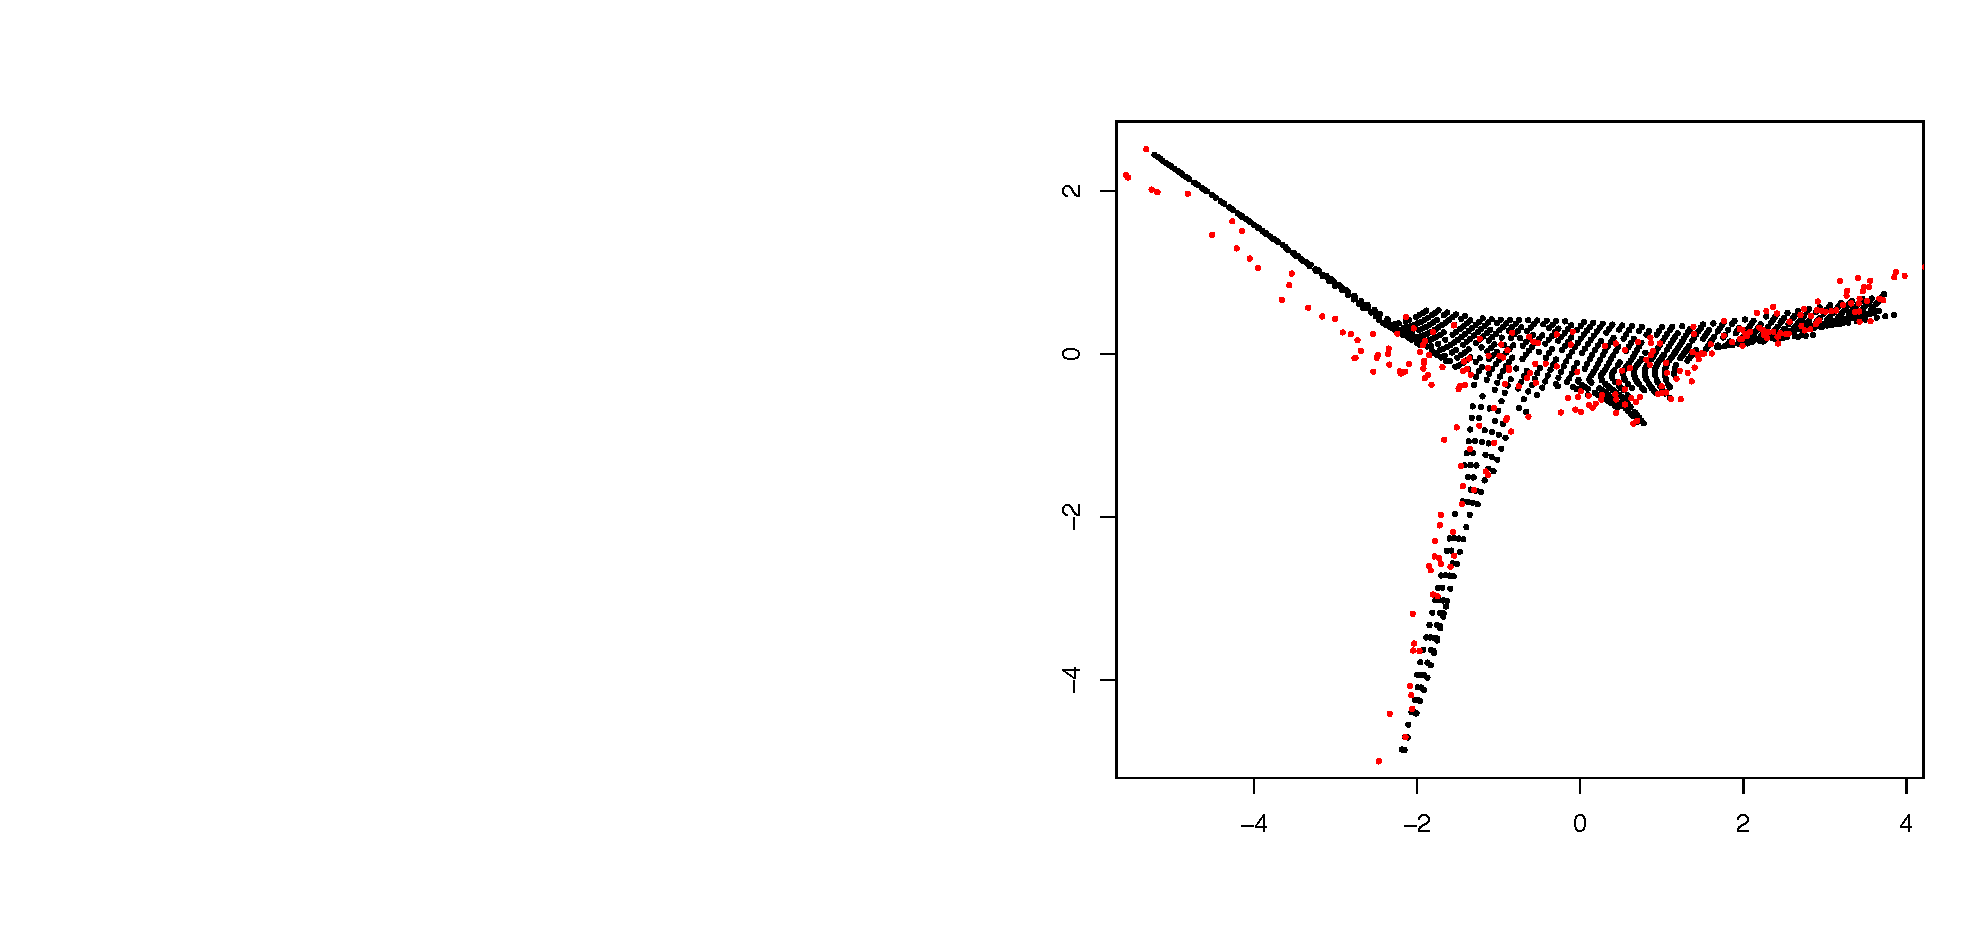
\includegraphics[width=4in]{figs/online-gowererror.pdf} \\
\caption{MDS configuration for the domain in \fig{wt2-grid-orig}. Black points are formed by the initial eigen-decomposition, where as the red points are positioned using Gower's interpolation online. The red points should be positioned in the ``holes'' in the black grid.}
\label{gowererror}
\end{figure}


Following from this, it is important to make sure that the MDS space is smooth in the sense that a grid of straight lines over the domain is mapped to a series of smooth lines. Taking the evenly spaced grid in \fig{wt2-grid-orig}, first MDS is performed on a dense point set of size 1253, and then a less dense grid is inserted using the method of Gower. The grid produced under the insertion can be seen in \fig{wt2-grid-full}. Taking a sample of 250 points from the 1253, an MDS configuration was also found and the same grid inserted (see \fig{wt2-grid-samp}.) From this it is clear that those points mapped into the domain are smooth but in the sample case the features in the far right of the shape (the less pronounced peninsulae) are squashed down.



% grid to map
\begin{figure}
\centering
% trim order l b r t
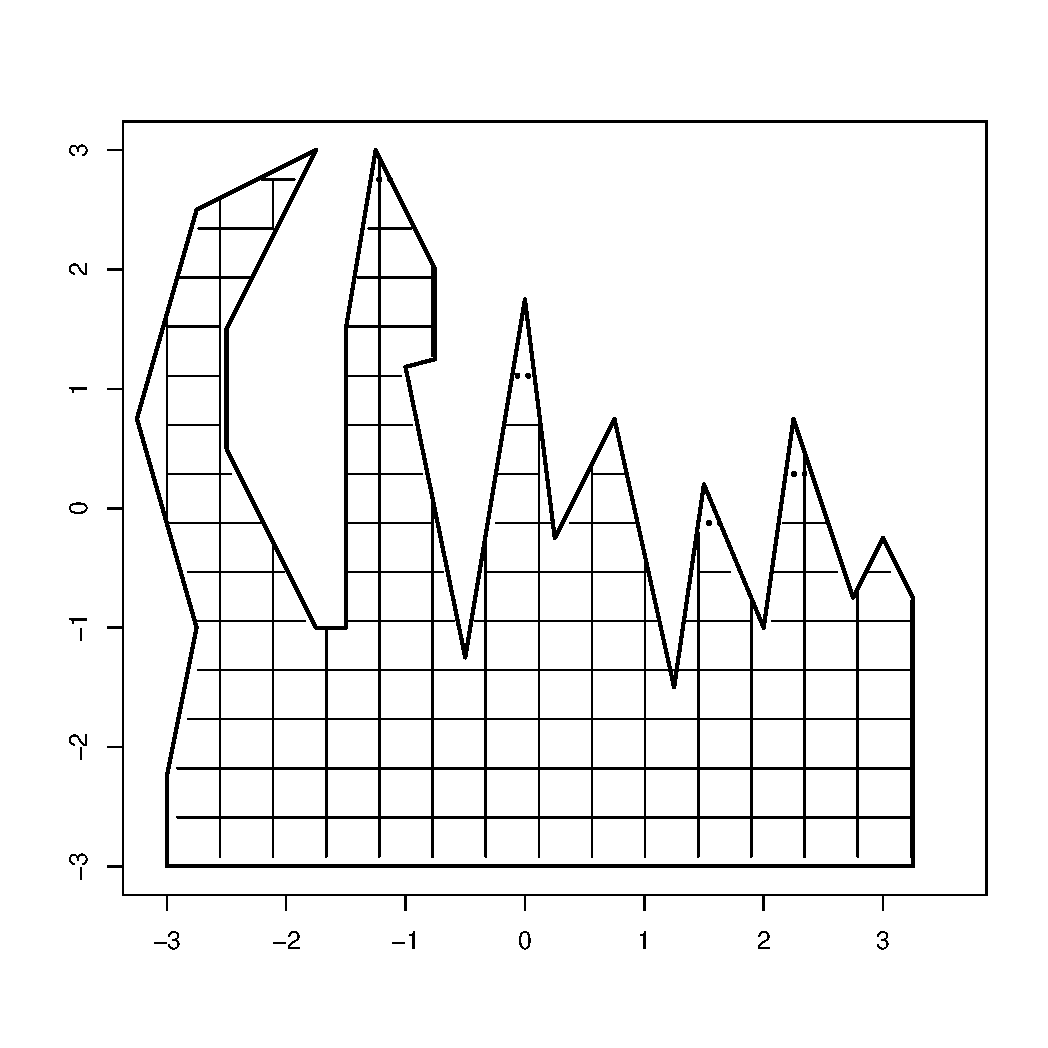
\includegraphics[width=4in]{figs/wt2-grid-orig.pdf} \\
\caption{The grid to be inserted into the MDS configuration.}
\label{wt2-grid-orig}
% generated using wt2-grid.R
\end{figure}

% mapped grid (full)
\begin{figure}
\centering
% trim order l b r t
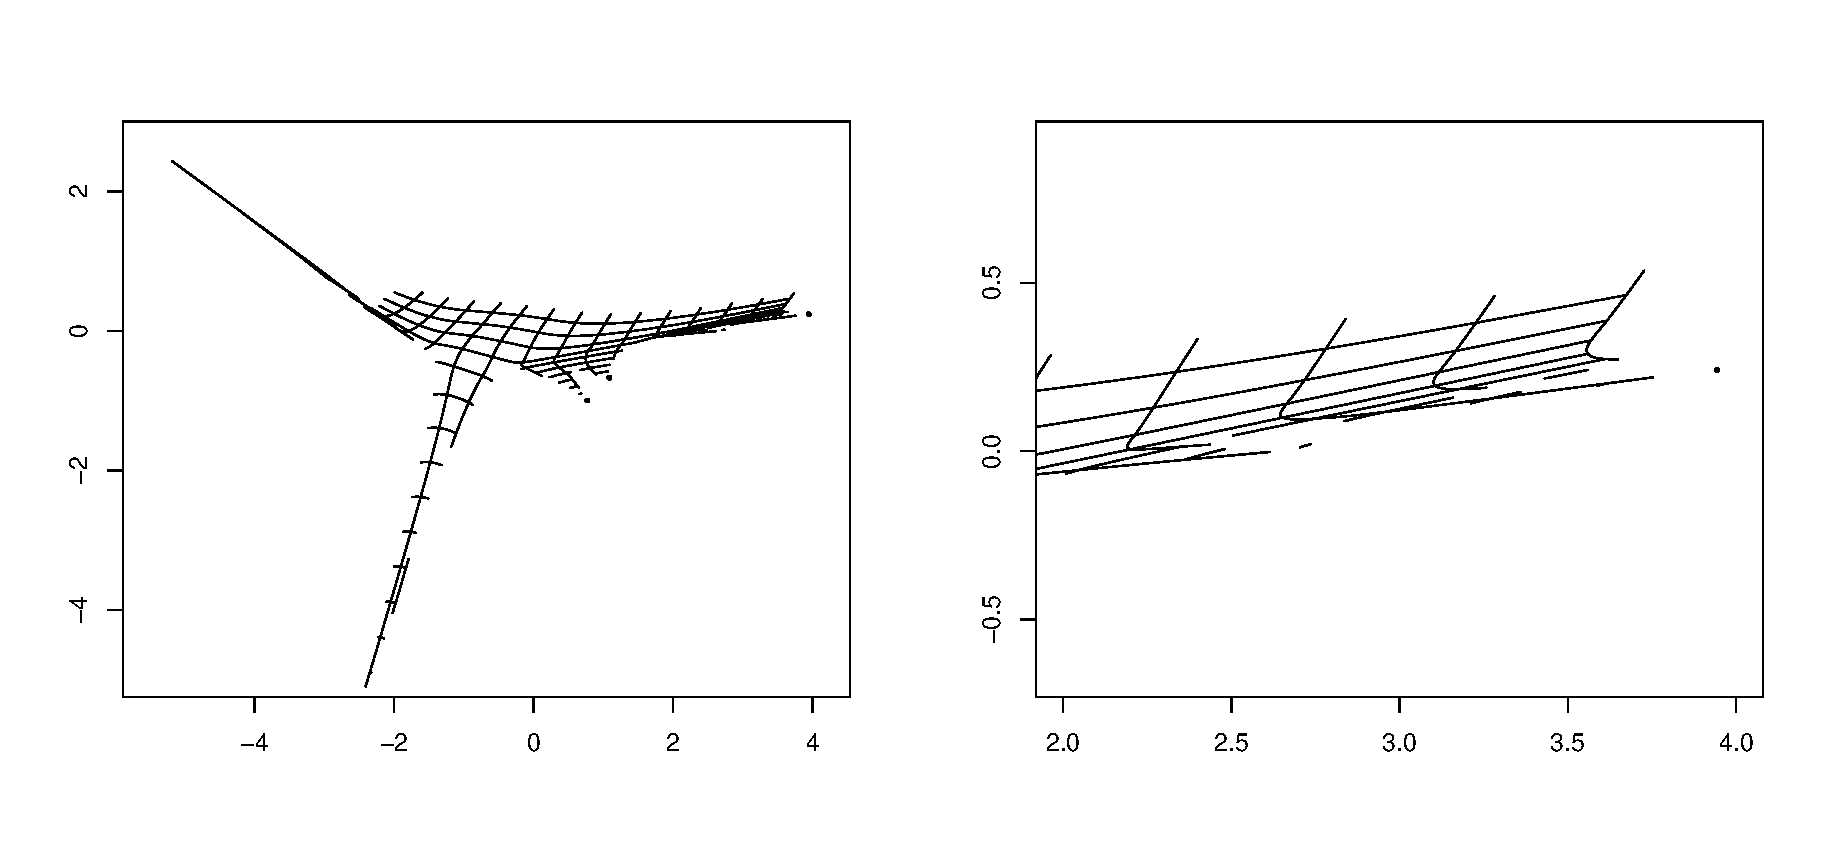
\includegraphics[width=5in]{figs/wt2-grid-full.pdf} \\
\caption{Inserted grid when 1253 points are used to create the initial MDS configuration. The right panel shows a zoom of the far right part of the configuration.}
\label{wt2-grid-full}
% generated using wt2-grid.R
\end{figure}

% mapped grid (samp)
\begin{figure}
\centering
% trim order l b r t
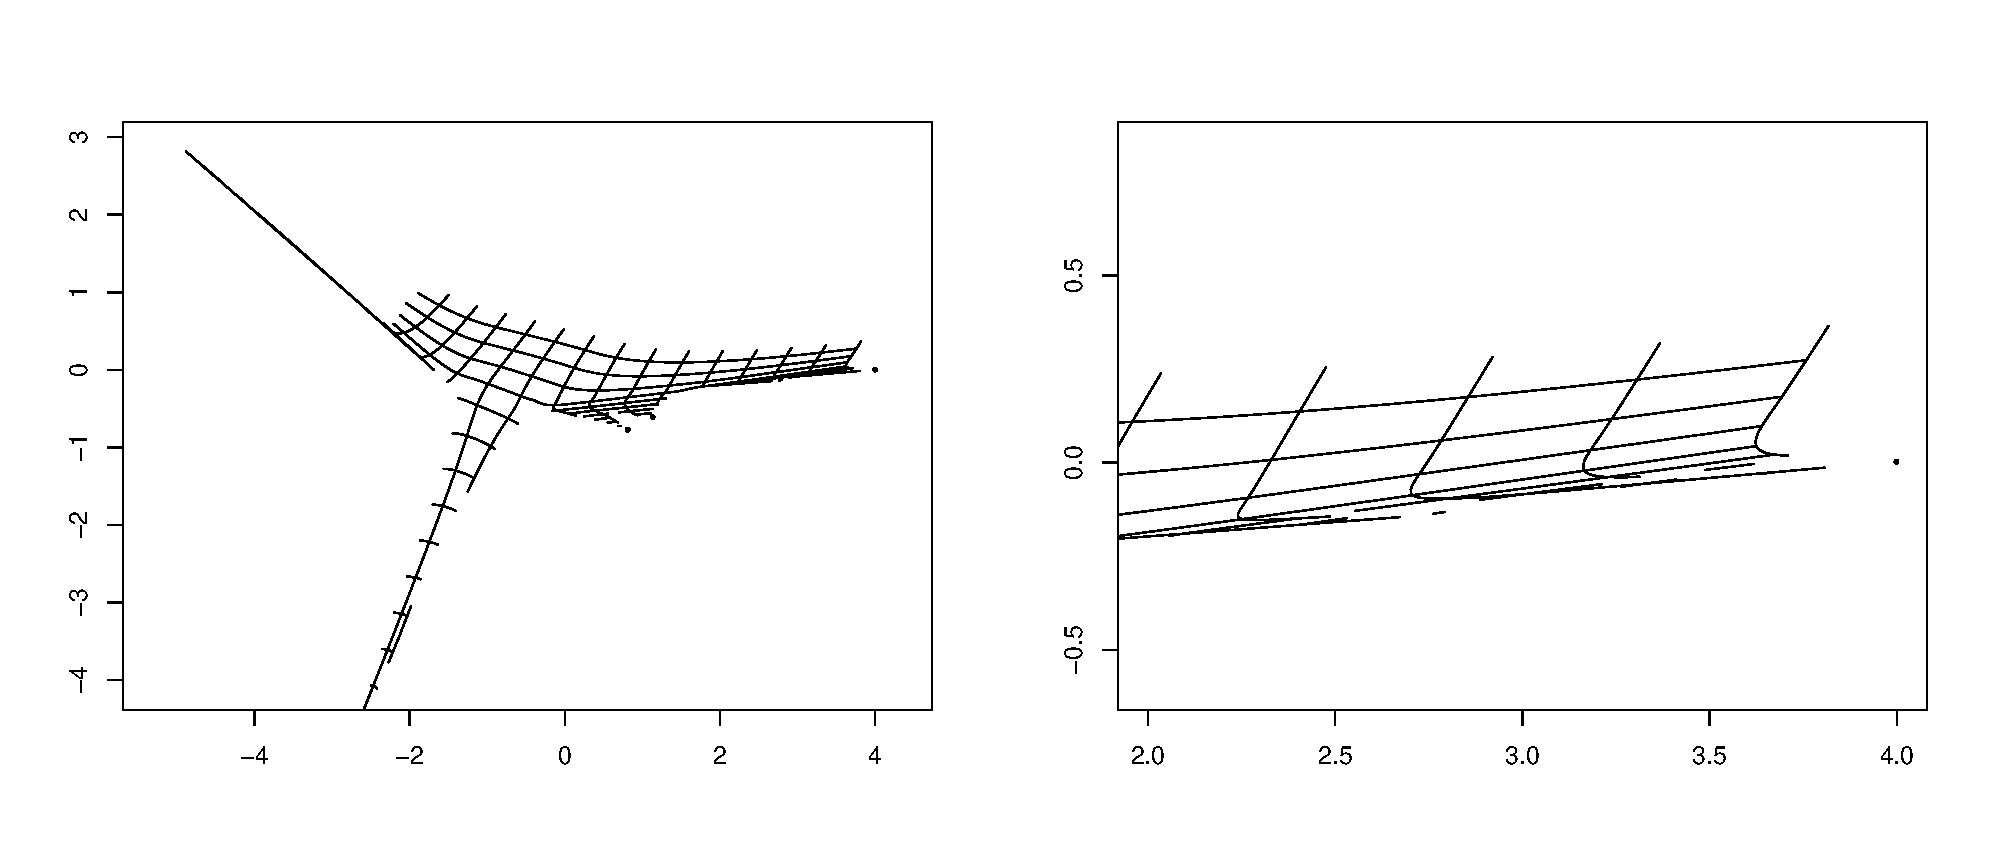
\includegraphics[width=5in]{figs/wt2-grid-samp.pdf} \\
\caption{Inserted grid when 250 randomly chosen points are used to create the initial MDS configuration. The right panel shows a zoom of the far right part of the configuration. Comparing this to that of \fig{wt2-grid-full}, one can see that the right side features have been squashed together.}
\label{wt2-grid-samp}
% generated using wt2-grid.R
\end{figure}

% wt2 with prediction and sample inserted
\begin{figure}
\centering
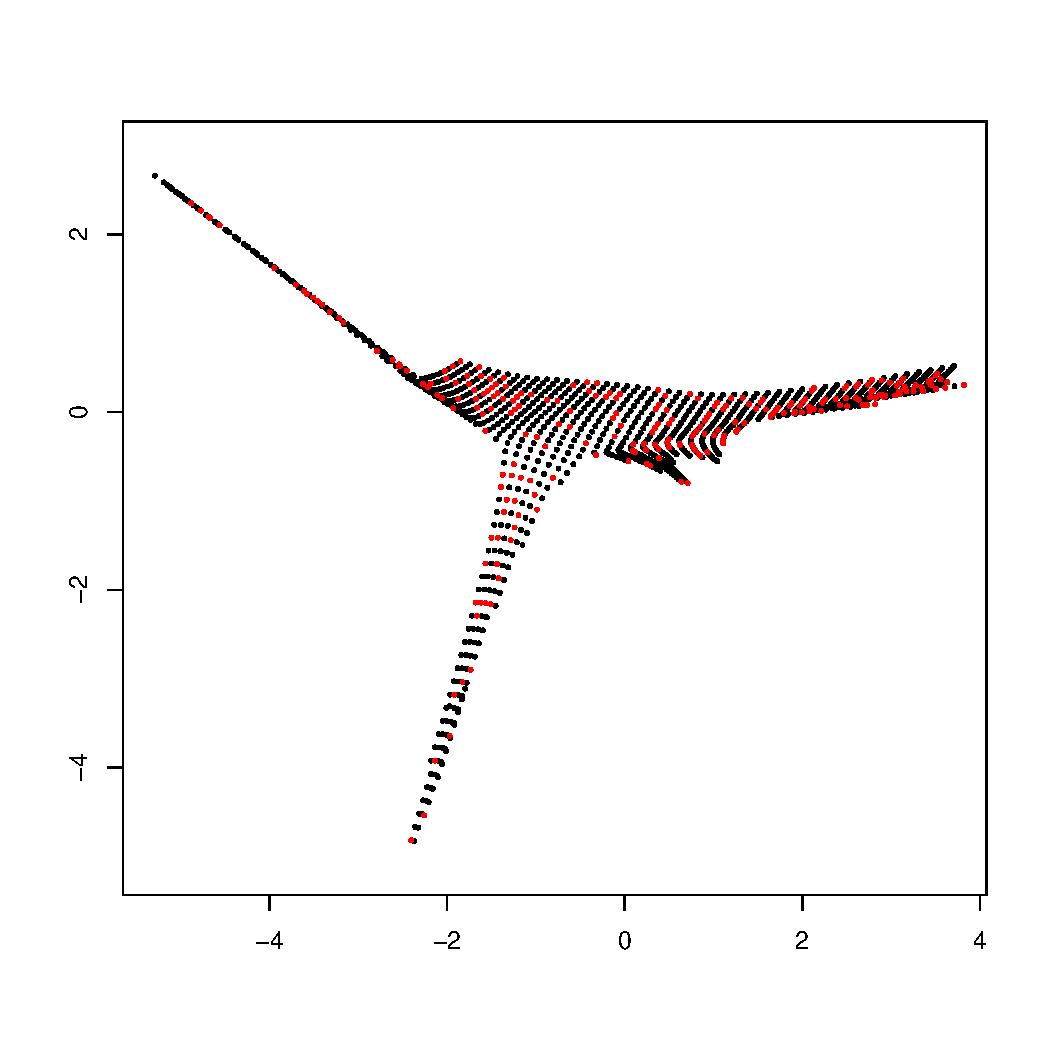
\includegraphics[width=4in]{figs/wt2-double-insert.pdf} \\
\caption{Here both black and red points were inserted into an MDS configuration of a 1007 point, evenly spaced grid over the domain. Both point sets are consistent.}
\label{wt2-double-insert}
% generated (roughly) using wt2-smooth-test.R
\end{figure}


\section{Finding the within-area distances}

In order to perform multidimensional scaling the matrix of distances must be first found. In this case it makes sense to find the shortest distances between each pair of points.

Thinking of the boundary of the domain as a polygon, the within-area distances are found by tracing the edges of this polygon from the first point to the second. The path between the points is then modified by deleting and replacing segments of it. Put more mathematically:

Given that there is no direct path ($\mathcal{P}$) within the domain ($\Gamma$, say) between two points ($p_1$ and $p_2$, say), the algorithm proceeds as follows:

\begin{enumerate}
\item Draw a line between $p_1$ and $p_2$ (\fig{wdia}, ($i$)). Start the path as the lines from $p_1$, $p_2$ to their first intersection with the boundary of $\Gamma$. Then find the distance between these two intersection points in both directions, along the boundary (\fig{wdia}, ($ii$).) Choose the shorter of these, add the paths between $p_1$, $p_2$ and the boundary and this is the starting path, $\mathcal{P}$ (\fig{wdia}, ($iii$).) 
\item Given a triple of vertices, $(v_i, v_{i+1}, v_{i+2}) \in \mathcal{P}$ , if the line between $v_i$ and $v_{i+2}$ is shorter than the path $(v_i, v_{i+1}, v_{i+2})$ and the line between $v_i$ and $v_{i+2}$ lies inside $\Gamma$ then delete $v_{i+1}$ (\fig{wdia}, ($iv$) and ($vi$).) This iterates over the entire path once, deleting all superfluous vertices. For example in \fig{wdia}, ($iii$) $v_2$ is deleted from $\mathcal{P}$ because the path straight between $v_1$ and $v_3$ is shorter. 
\item Given a triple of vertices, $(v_i, v_{i+1}, v_{i+2})$ if the path $(v_i, \text{some subset of the vertices of } \Gamma, v_{i+2})$ is shorter than the path $(v_i, v_{i+1}, v_{i+2})$ then replace $v_{i+1}$ with those elements of $\Gamma$ (\fig{wdia}, ($v$)). For example in \fig{wdia} ($iv$), the path $(v_1, v_2, v_3)$ is longer than the path $(v_1, v^1_1, v^1_2, v^1_3, v_3)$ so the former is replaced with the latter in $\mathcal{P}$.
\item We then iterate between steps 2 and 3 until there has been no change from one run to the next (ie. convergence) or there have been too many iterations (\fig{wdia}, ($vi$).)
\end{enumerate}

% diagram for finding the shortest path in W
\begin{sidewaysfigure}
\centering
% trim order l b r t
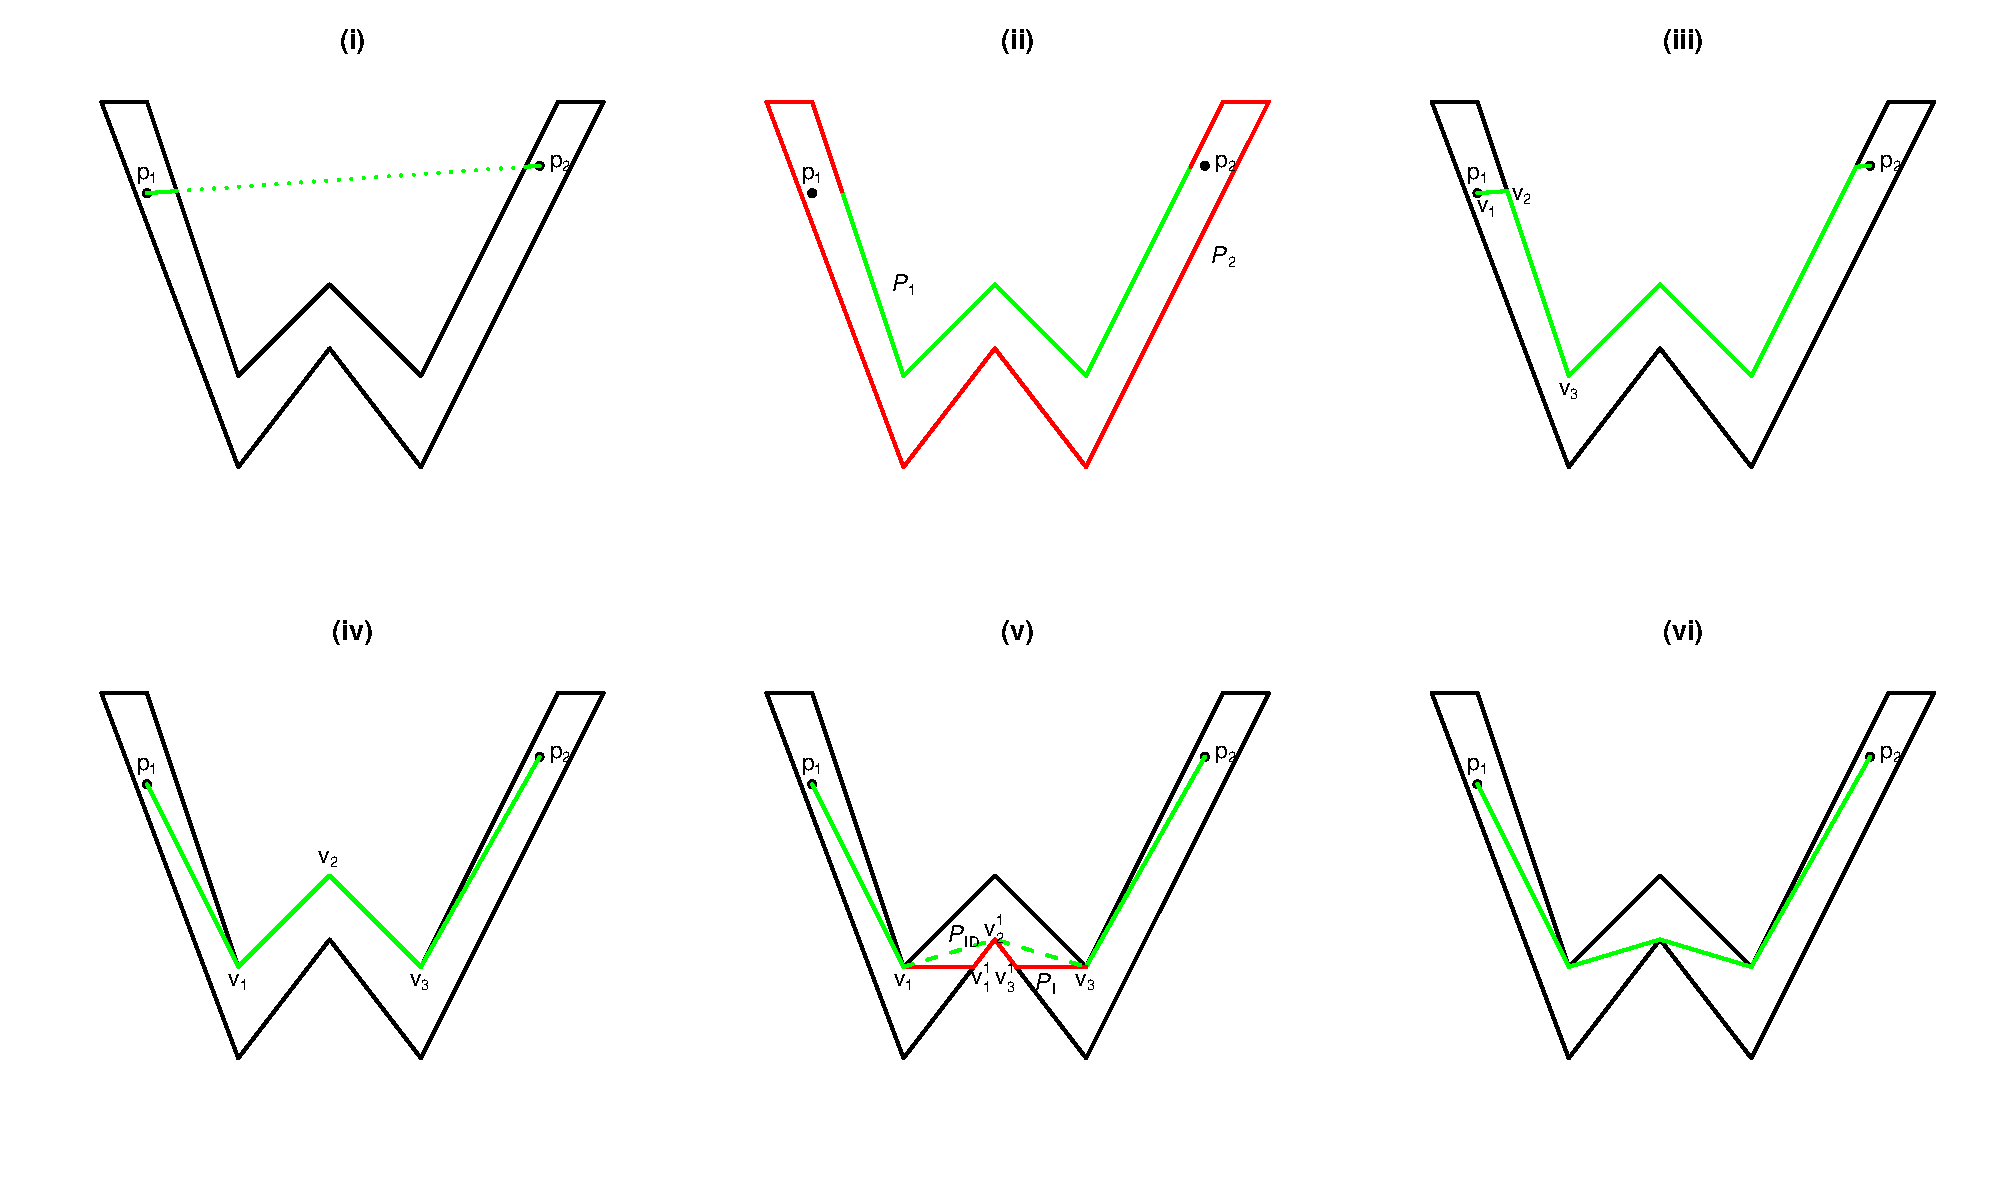
\includegraphics[trim=0in 0.5in 0in 0.25in, width=9.5in]{figs/wdia.pdf} \\
\caption{The green lines in ($i$) to ($vi$) show the path as the algorithm progresses from initial state to final, shortest path (bottom right.) }
\label{wdia}
% generate /phd-smoothing/mds-writeup/figs/distanceexplanation.R
\end{sidewaysfigure}

Of course, if there is a direct path between $p_1$ and $p_2$ the the Euclidean distance between the points can be used.

\section{Multidimensional scaling for smoothing over complex domains}

Taking a cue from \cite{soap} simulations were conducted on the so-called modified Ramsay horseshoe and another domain supposed to mimic that of a coastline.

\subsection{Modified horseshoe}

For the modified horseshoe (\fig{leakage}), 100 replications of samples of 250 points with normal errors (at 3 levels) were run. From these samples, three models were fit to the data and predictions over 718 points (including the sample locations) and the mean squared error was calculated between the model prediction and the true function value for the horseshoe. The three models fit were as follows using the \textsf{R} packages \texttt{mgcv} and \texttt{soap}:

\begin{enumerate}
\item \emph{Thin plate spline}: bivariate thin plate spline with basis size 100.
\item \emph{Soap film smoother}: 32 knots evenly spread over a grid over the domain, cyclic spline on the boundary was of basis size 39.
\item \emph{MDS}: Used a thin plate spline of basis dimension 100.
\end{enumerate} 

As can be seen from \fig{ramsay-fit-1}

\begin{table}[ht]
\centering
\begin{tabular}{c || c c c}
$\sigma^2$ & MDS & Soap film & Thin plate\\ 
\hline
0.1  & 0.0032 (0.0004) & 0.0022 (0.0004) & 0.0402 (0.0123)\\ 
1  & 0.0436 (0.0233) & 0.0482 (0.0222) & 0.2306 (0.0383)\\ 
10  & 2.0652 (1.9208) & 3.0702 (3.7669) & 3.3713 (1.7916)\\ 
\end{tabular}
\label{ramsayresultstable}
\caption{}
\end{table}

% Ramsay fit with error=1 
\begin{figure}
\centering
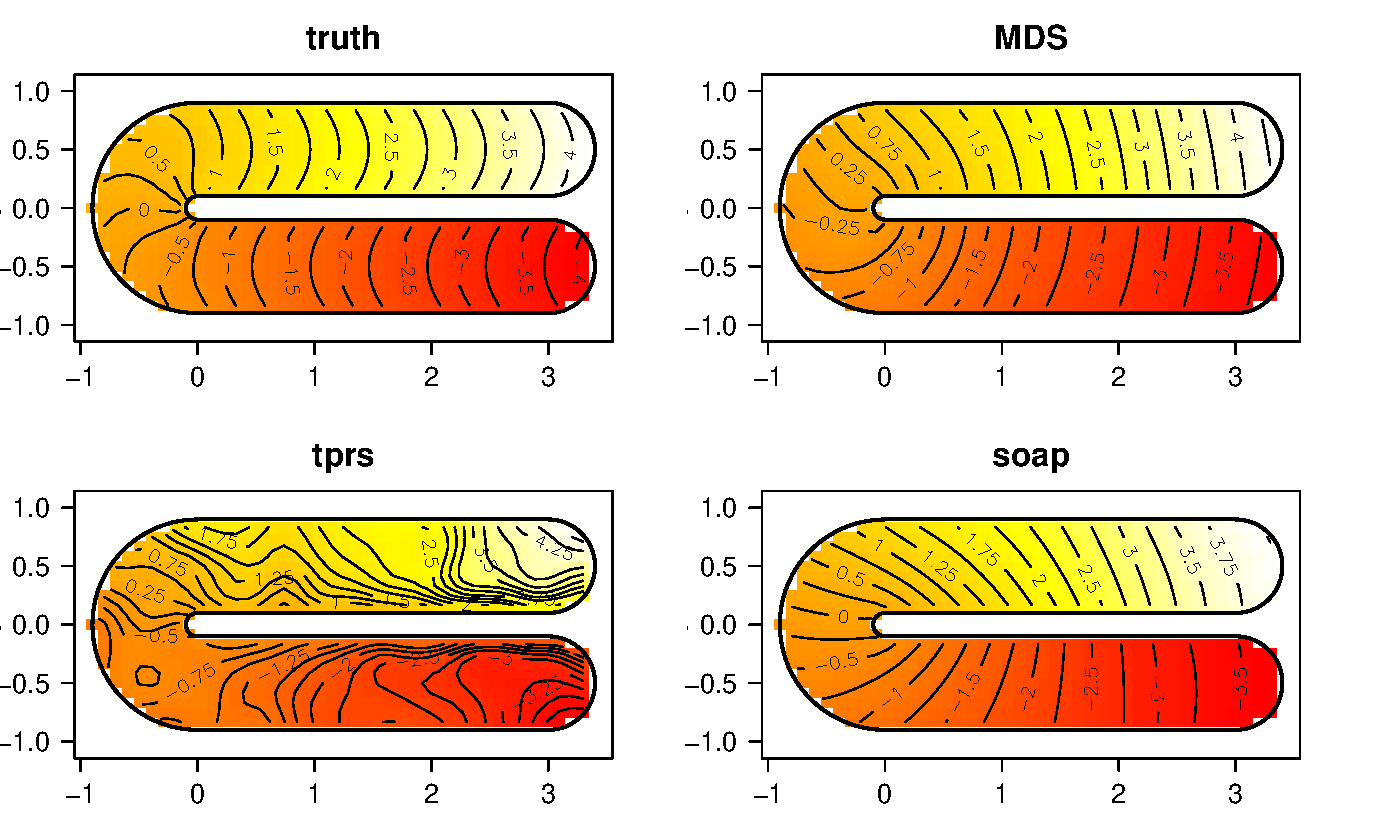
\includegraphics[width=6in]{figs/ramsay-fit-1.pdf} \\
\caption{}
\label{ramsay-fit-1}
% generated (roughly) using ramsay-smooth-test.R
\end{figure}

\subsection{Peninsulae domain}

The Ramsay horseshoe is, in a sense, easy domain to smooth over since it is obvious what the transformation should be doing. For this reason a more complex and more realistic domain would provide more insights into the efficacy of the method. The domain shown in \fig{wt2-truth} is an approximation to a coastline with a strong trend along both peninsulae (in a manner similar to that of the horseshoe) but with the added complication of a further peak in the lower right corner.

Again, 100 realisations from the domain shown in \fig{wt2-truth} were used with Normal errors at 3 levels of $\sigma^2$. Mean squared error over 1253 prediction points was calculated from fitting models with 250 samples. The models fit were:

% wt2 truth 
\begin{figure}
\centering
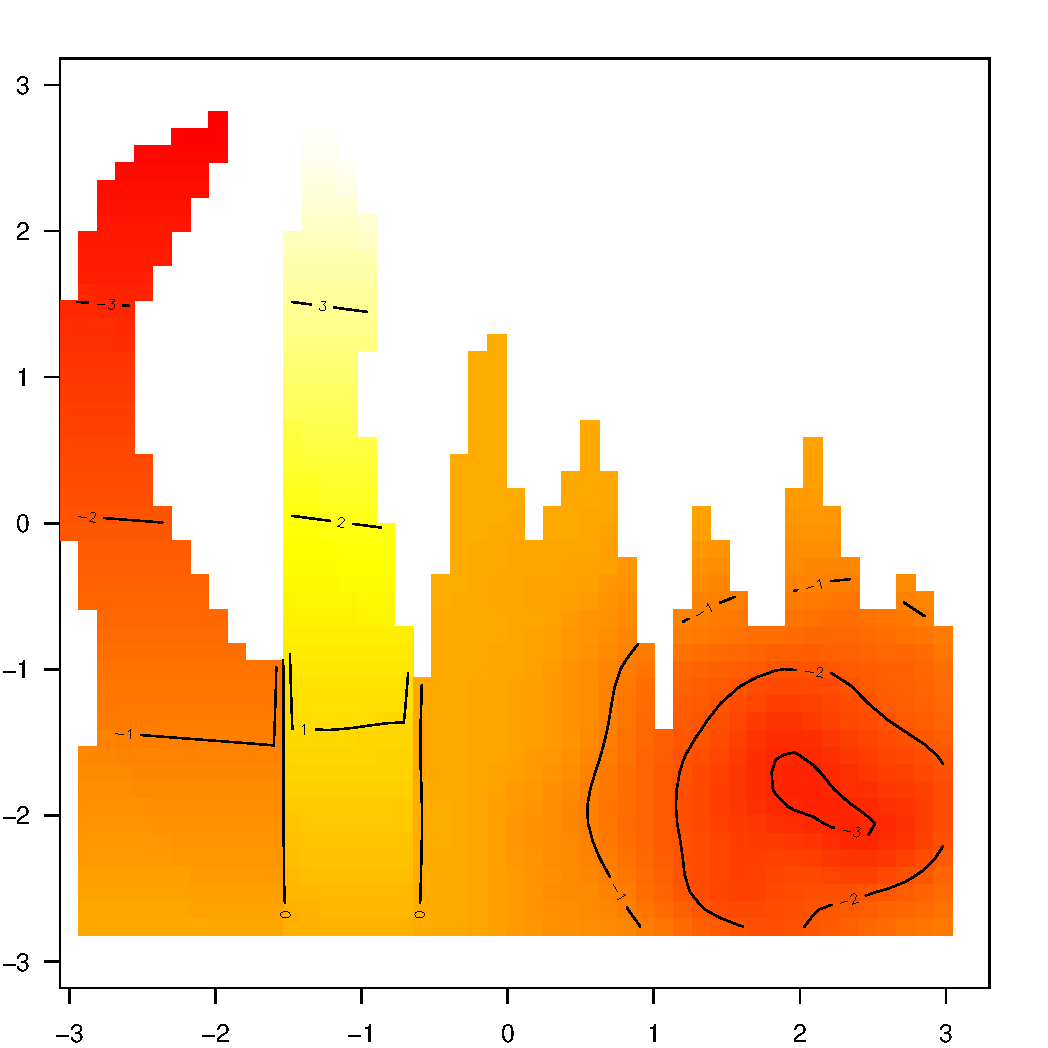
\includegraphics[width=3in]{figs/wt2-truth.pdf} \\
\caption{True function for the domain with multiple peninsulae.}
\label{wt2-truth}
% generated (roughly) using wt2-smooth-test.R
\end{figure}

\begin{enumerate}
\item \emph{Thin plate spline}: bivariate thin plate spline with basis size 100. 
\item \emph{Soap film smoother}: cyclic spline on boundary of basis size 60, 109 internal knots evenly spaced over the domain on a grid.
\item \emph{MDS}: after transform a thin plate spline with basis size 100 was fit. 
\item \emph{MDS with tensor product}: tensor product of two thin plate splines, each of basis dimension 12.
\end{enumerate} 

The final option was chosen after it appeared that the MDS with a bivariate thin plate spline did not adequately model the peak in the right corner of the domain see [FIG panel blah]. After using a tensor product of thin plate splines a better fit to the right peak was found (see [FIG panel], although this is not reflected particularly well in terms of mean squared error (see table \ref{wt2resultstable}.) The visual improvement in fit can be explained by thin plate splines in two dimensions being an isotropic smooth and since space has not been transformed in a uniform way in both dimensions (see [FIG].)

\begin{table}[ht]
\centering
\begin{tabular}{c || c c c c}
$\sigma^2$ & MDS & MDS (tensor) & Soap film & Thin plate\\ 
\hline
0.05 & 0.0965 (0.0132) & 0.0643 (0.0681) & 0.0249 (0.0078) & 0.0525 (0.0223)\\ 
0.5 & 0.1425 (0.0128) & 0.1111 (0.0293) & 0.0826 (0.102) & 0.1128 (0.0273)\\ 
5 & 0.9102 (0.4768) & 1.2509 (0.9372) & 1.1544 (0.6089) & 1.3853 (0.4799)\\ 
\end{tabular}
\label{wt2resultstable}
\caption{}
\end{table}

% wt2 fit with error=0.5
\begin{figure}
\centering
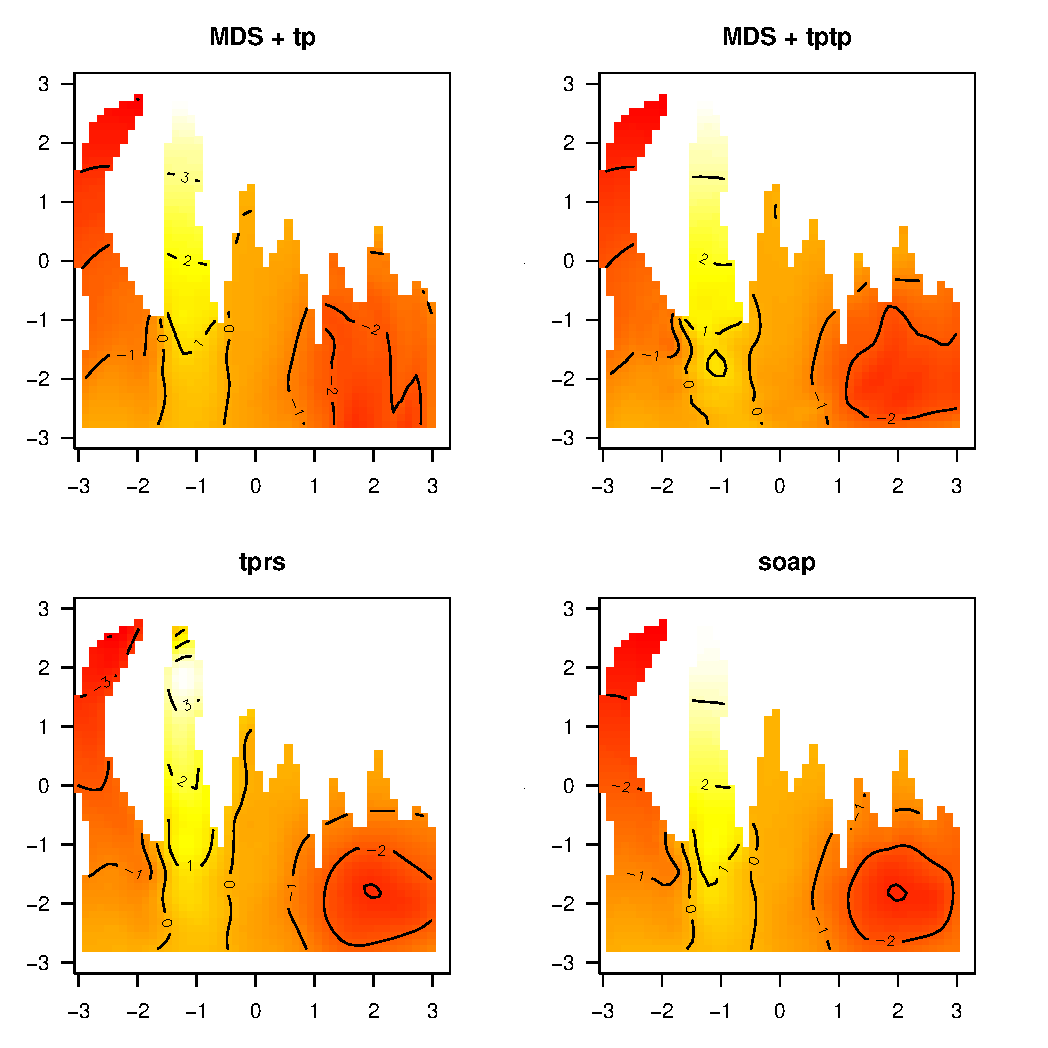
\includegraphics[width=6in]{figs/wt2-fit-005.pdf} \\
\caption{A typical realisation of fits from the multiple peninsulae domain when $\sigma^2$ is set to 0.05.}
\label{wt2-fit-0.05}
% generated (roughly) using wt2-smooth-test.R
\end{figure}



\section{Conclusions}

Although these results are encouraging, the inability of the smooth to capture the features in the right side of the domain when an isotropic smoother is disappointing. Proposed further work is to follow the lead from \cite{wood2000}, which shows that given some transform of a variable, $y$ say, such that $y_i^\prime=y_i/k$, then $f(x,y^\prime k)$ will give the same fit as $f(x,y)$ (ie. the fit will be the same under the new coordinates) but the penalty will change to:
\begin{equation}
\int\int_\Omega \Big( \frac{\partial^2 f}{\partial x^2} \Big) + 2k\Big( \frac{\partial^2 f}{\partial x \partial y} \Big) + k^3\Big( \frac{\partial^2 f}{\partial y^2} \Big) \text{d}x \text{d}y,
\label{adjustedintegral}
\end{equation}
from:
\begin{equation*}
\int\int_\Omega \Big( \frac{\partial^2 f}{\partial x^2} \Big) + 2\Big( \frac{\partial^2 f}{\partial x \partial y} \Big) + \Big( \frac{\partial^2 f}{\partial y^2} \Big) \text{d}x \text{d}y.
\end{equation*}
In the case of the MDS, the integral would need to be split over a grid such that each cell captured the distortion in space over the area of the cell. Mathematically, $\Omega$ would be split into a subsets, $\omega_i$ (where $\bigcup_{\forall j} \omega_j = \Omega$) and (\ref{adjustedintegral}) becomes:
\begin{equation}
\sum_{\forall j} \int\int_{\omega_j} l_j^3 \Big( \frac{\partial^2 f}{\partial x^2} \Big) + 2k_jl_j\Big( \frac{\partial^2 f}{\partial x \partial y} \Big) + k_j^3\Big( \frac{\partial^2 f}{\partial y^2} \Big) \text{d}x \text{d}y,
\end{equation}
where $k_j$ is the scaling in the $y$ direction and $l_j$ is the scaling in the $x$ direction for the $j^{\text{th}}$ cell. We assume here that $f(x,y)$ is ``nice''.

Using this penalty may allow for the distortions in space to be taken account of and therefore get around the problem of the details being smoothed over, as seen above. It will be easiest to first build this using a tensor product of $P$-splines to test its utility (since their penalty is discrete) and then move on to the thin plate spline penalty.

Finally, in order to make this technique competitive with \texttt{soap} (assuming that the above distortion adjustment is successful) a speed-up in the computation of the within-area distances must be achieved. At the moment this is the major bottleneck in the calculation since model fitting consists only of fitting a thin plate spline. 

Speed-ups can be achieved by minimizing the number of calculations for within-area distance that are needed. In \cite{landmark} a method to calculate MDS coordinates using a sparse grid of landmark points is suggested; although the authors are sceptical about how this will perform with non-Euclidean distances. There is clearly some work here in finding some minimal set of landmark points for the within-area distance metric obtained from the above algorithm.

The calculation of within-area distances could be linked into a ``landmark''-type process by calculating the within-area distances between a set of points in a sparse grid, then saving those paths. The distances between desired points can then be found by modifying the path with the end points nearest to those of the desired points.


\bibliographystyle{plainnat}
\bibliography{mds-refs}

\end{document}
